% Created 2021-09-11 Sat 09:35
% Intended LaTeX compiler: xelatex
\documentclass[letterpaper]{article}
\usepackage{graphicx}
\usepackage{grffile}
\usepackage{longtable}
\usepackage{wrapfig}
\usepackage{rotating}
\usepackage[normalem]{ulem}
\usepackage{amsmath}
\usepackage{textcomp}
\usepackage{amssymb}
\usepackage{capt-of}
\usepackage{hyperref}
\usepackage[margin=1in]{geometry}
\usepackage{fontspec}
\usepackage{indentfirst}
\setmainfont[ItalicFont = LiberationSans-Italic, BoldFont = LiberationSans-Bold, BoldItalicFont = LiberationSans-BoldItalic]{LiberationSans}
\newfontfamily\NHLight[ItalicFont = LiberationSansNarrow-Italic, BoldFont       = LiberationSansNarrow-Bold, BoldItalicFont = LiberationSansNarrow-BoldItalic]{LiberationSansNarrow}
\newcommand\textrmlf[1]{{\NHLight#1}}
\newcommand\textitlf[1]{{\NHLight\itshape#1}}
\let\textbflf\textrm
\newcommand\textulf[1]{{\NHLight\bfseries#1}}
\newcommand\textuitlf[1]{{\NHLight\bfseries\itshape#1}}
\usepackage{fancyhdr}
\pagestyle{fancy}
\usepackage{titlesec}
\usepackage{titling}
\makeatletter
\lhead{\textbf{\@title}}
\makeatother
\rhead{\textrmlf{Compiled} \today}
\lfoot{\theauthor\ \textbullet \ \textbf{2021-2022}}
\cfoot{}
\rfoot{\textrmlf{Page} \thepage}
\titleformat{\section} {\Large} {\textrmlf{\thesection} {|}} {0.3em} {\textbf}
\titleformat{\subsection} {\large} {\textrmlf{\thesubsection} {|}} {0.2em} {\textbf}
\titleformat{\subsubsection} {\large} {\textrmlf{\thesubsubsection} {|}} {0.1em} {\textbf}
\setlength{\parskip}{0.45em}
\renewcommand\maketitle{}
\author{Houjun Liu}
\date{\today}
\title{Human Diseases}
\hypersetup{
 pdfauthor={Houjun Liu},
 pdftitle={Human Diseases},
 pdfkeywords={},
 pdfsubject={},
 pdfcreator={Emacs 27.2 (Org mode 9.4.4)}, 
 pdflang={English}}
\begin{document}

\maketitle


\section{Overview of Human Diseases}
\label{sec:org97a29c6}
A lecture by the Legendary Dr. Paul Hauser.
\href{https://docs.google.com/presentation/d/1b2RetU6iGsd\_h4Msb2SV-\_WznNXSREbsPpfdY-LgJZs/edit\#slide=id.ga6d683dbbf\_0\_338}{Slides
are here}

\#flo \#disorganized

\textbf{Disease} is an abnormal condition that causes impairment in/loss of
function of an organism (a.k.a. decreased fitness) that is not due to
immediate external injury.

\begin{itemize}
\item What causes human disease?

\begin{itemize}
\item Infectious agents
\item Deficiency disorders
\item Heritable factors
\item Physiological disorders (immunodeficiency, autoimmune disorders,
allergies, etc.)
\end{itemize}
\end{itemize}

\subsection{Congenital vs. Acquired disease}
\label{sec:org3e316b6}
Congenital diseases => diseases present at birth due to DNA
abnormalities / pregnancy pathological issues

Acquired diseases => diseases that begin during lifetime, including\ldots{}

\begin{itemize}
\item Microrganism invasion => "infectios diseases"
\item Autoimmune reaction
\item Nutrient deficiency
\item Mechanical wear
\item Ingestion of noxious chemicals
\end{itemize}

\textbf{Infectious diseases actually smaller on the causes of death in the US}

\begin{itemize}
\item Heart disease => wear + deficiency
\item Cancer => heritable + DNA
\item Unintentional injuries => not a disease
\item Chronic respitory disease => wear
\item Stroke => not a disease
\item Alhetimer disease => wear
\item Diabetes => autoimmune, nutrient, wear
\item Influenca <= \textbf{here, finally, an infections disease.}
\end{itemize}

\subsection{Disease causing agents}
\label{sec:org929053d}
\begin{itemize}
\item \textbf{Protozoan} => single-celled eukaryotes
\item \textbf{Fungal} => single/multi-celled eukarotyes
\item \textbf{Bacteria} => single-celled prokaryotes
\item \textbf{Viral} => acellular parasitic infectious agent
\item \textbf{Helminuthus} => multicellular worms
\item \textbf{Prions} => acellular misfolded proteins
\item \textbf{Viroids} => infections nucleic acids w/o protein coat to make virus
\end{itemize}

\subsection{Pathogenicity + Virulence}
\label{sec:org8abfa93}
\textbf{Pathoginecity} => relative capacity to cause disease

\begin{itemize}
\item Non-pathogenic agents => no diesease
\item Primary pathogens => yes disease
\item Opportunistic pathogens => yes disease only when it can, for instance,
in immunocompromised individuals
\end{itemize}

\textbf{Virulence} => numerical measures for pathonicity

\begin{itemize}
\item Measured experimentally with LD50 + ED50
\end{itemize}

\noindent\rule{\textwidth}{0.5pt}

\subsection{Overview of various diseases}
\label{sec:orgd53a4dc}
\href{https://drive.google.com/file/d/1WRnbgkhnmRrdP4ZqlqT3HHBD1\_eW9qib/view}{This
video}

\subsubsection{Protozoan}
\label{sec:orgab0a66e}
\begin{itemize}
\item \textbf{Protozoan factors} => direction pathogenisis leading to tissue damage
\item \textbf{Host-mediated factors} => immune evation + escape mechnisms +
immunalsupression
\end{itemize}

Adaptable!!

\subsubsection{Fungal}
\label{sec:orga85528e}
\begin{itemize}
\item \textbf{Fungal factors} => many shapes and very adaptable, colud produced
specialized enzymes to take root in body
\item \textbf{Host-mediated factors} => cause immunocomprimzation, acquired though
inhalation, etc.
\end{itemize}

\subsubsection{Bacteria}
\label{sec:orge331b6b}
\begin{itemize}
\item \textbf{Bacterial-induced toxicity} => produces toxins + has hard capsule
cell
\item \textbf{Host-mediated factors} => may develop host resistance, could compete
for resources, and could be grown introcellularly
\end{itemize}

\begin{figure}[htbp]
\centering
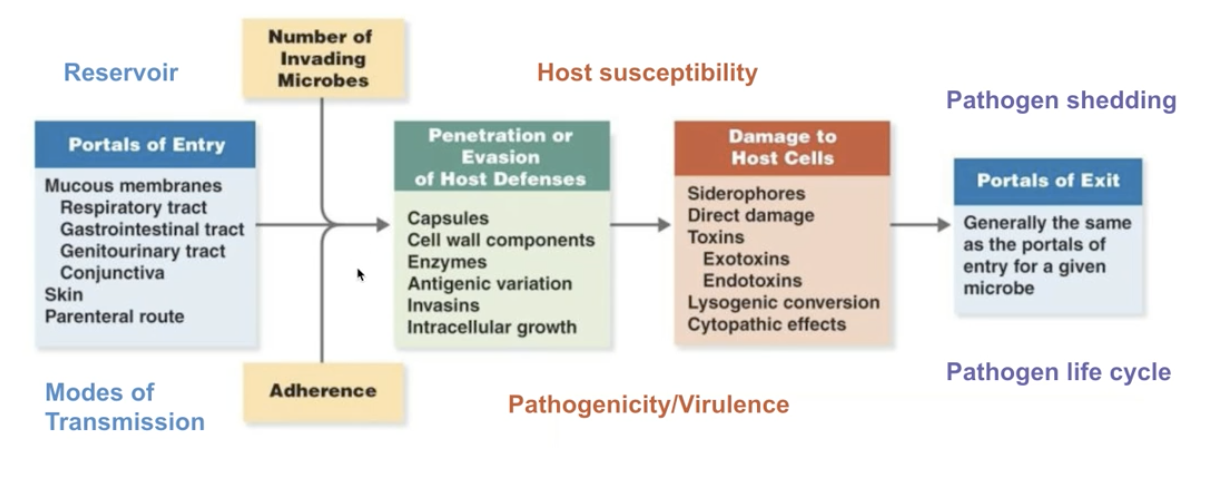
\includegraphics[width=.9\linewidth]{Screen Shot 2020-10-12 at 3.08.53 PM.png}
\caption{Screen Shot 2020-10-12 at 3.08.53 PM.png}
\end{figure}

\noindent\rule{\textwidth}{0.5pt}

\subsection{Bacteria causing diseases}
\label{sec:org0589801}
\textbf{Biofilm formation}

\begin{itemize}
\item Communities of bacteria could work together by adhering and exchanging
information
\item Bacterial could perform quorum sensing => exchange of information with
each other + recognize various members of their group
\end{itemize}

\subsubsection{Fighting bacterial infections}
\label{sec:org9df8ed0}
\textbf{Antibiotics} => drugs with selective toxicity for specific bacterial
types

Act by\ldots{}

\begin{itemize}
\item Disrupting membrane + cell wall integrity
\item Selectively target + impair bacterial ribosomes
\item Block bacterial DNA replication/transcription
\item Inhibit bacterial metabolism
\end{itemize}

\subsection{Viruses causing diseases}
\label{sec:orgf680af4}
\textbf{Viruses: acellular macromolecular assemblies}

\begin{itemize}
\item Contain protein coat called capsid

\item DNA or RNA, but not both

\item Are obligate parasites that could only replicate within host

\item Assembled and mature viral particles => virions, which contain\ldots{}

\begin{itemize}
\item Capsid
\item Genetic material
\item Occationally outside lipid layer
\end{itemize}
\end{itemize}

=> Viruses exist on the nanometre scale, but they are difference in
share and size

\subsubsection{Structure of viruses}
\label{sec:org243bbcc}
\begin{itemize}
\item \textbf{All contain}

\begin{itemize}
\item Capsid => structural protein coat
\item Genome => RNA/DNA; but not both
\end{itemize}

\item \textbf{Some contain}

\begin{itemize}
\item Membraneous-enclosed capsid => envelope
\item Externally-facisg host-cell fusion proteins => spikes
\item Viral genome replication enzymes => prlymerases
\item Other proteins for fun => enzymes, motor proteins, transcription
factors, host-cell interacting proteins, etc.
\end{itemize}
\end{itemize}

\subsubsection{Two types of virus}
\label{sec:orgda68f95}
\begin{itemize}
\item \textbf{Prokaryotic-infecting viruses}

\begin{itemize}
\item Variety of shapes
\item Complex and prolate shapes
\item Has, sometimes complex shapes! a la
\href{Screen Shot 2020-10-12 at 10.49.04 PM.png}{this
image}
\end{itemize}

\item \textbf{Eukarotic-infecting viruses}

\begin{itemize}
\item Much more "boring" in terms of shape
\item Icosahedral/spherecial outside
\item Enveloped constructions => envelope protein layer outside, spherical
inside
\item Helical/Cylindrical/Bullet shapes, too!
\item Often single patterns assemble together to create symmetric shape
that creates the whole of the virus
\end{itemize}
\end{itemize}

\subsubsection{Viral Life Cycle}
\label{sec:org0f7ba76}
\begin{enumerate}
\item Attachment => protein contact between virus and host
\item Viral entry/Uncoating => shedding the protein layer
\item Biosynthesis => make baby viruses

\begin{enumerate}
\item Genome Replication: transcribe DNA/RNA
\item Genome Expression: read DNA/RNA to make proteins
\end{enumerate}

\item Viral genome integration => retrovirus only
\item Assembly => put it all togethr
\item Viral Exit => mature virons leave
\end{enumerate}

\begin{enumerate}
\item Viral Entry
\label{sec:org979b8d7}
\emph{Option 1: Direct Injection/insertion}

\begin{itemize}
\item Insert genome through the bi-layer
\item Leave the rest behind
\item Tada!
\end{itemize}

\emph{Option 2: Endocytosis}

\begin{itemize}
\item Trick the host cell into introducing the virus as food
\item Endocytosis!
\item Bam
\end{itemize}

\emph{Option 3: Fusion}

\begin{itemize}
\item Virus fuse with cell membrane
\item Shed the protein coat once in
\item Shazam!
\end{itemize}

\textbf{All of these involve attachment first, which usually takes two steps.}

This process causes the organism-specific response to viruses:

\begin{enumerate}
\item Attachment: adhere roughly to random sugar proteins
\item Binding: roll over slowly, and bind to the entry receptor it needs
\end{enumerate}

\item Uncoating
\label{sec:orgf004954}
\begin{itemize}
\item Virus triggers \emph{early endosome}

\begin{itemize}
\item Causes pH dependent protein denaturation
\item Causing the capsid to fall apart
\item Triggering \emph{late endosome} => releasing genome
\end{itemize}
\end{itemize}

\item Viral Replication
\label{sec:orgc00d245}
Key questions:

\begin{itemize}
\item \textbf{How are viral mRNAs produced from the viral genome?} => virus will
hijack the ribosomes in the host cells. So, it is more important to
ask how the mRNAs are produced to tell ribosomes what to do
\item \textbf{What serves as the template for viral genome replication} =>
replication will need a polymeraese; but the source and mechanism is
dependent on viral genome structure/composition
\end{itemize}

\begin{figure}[htbp]
\centering
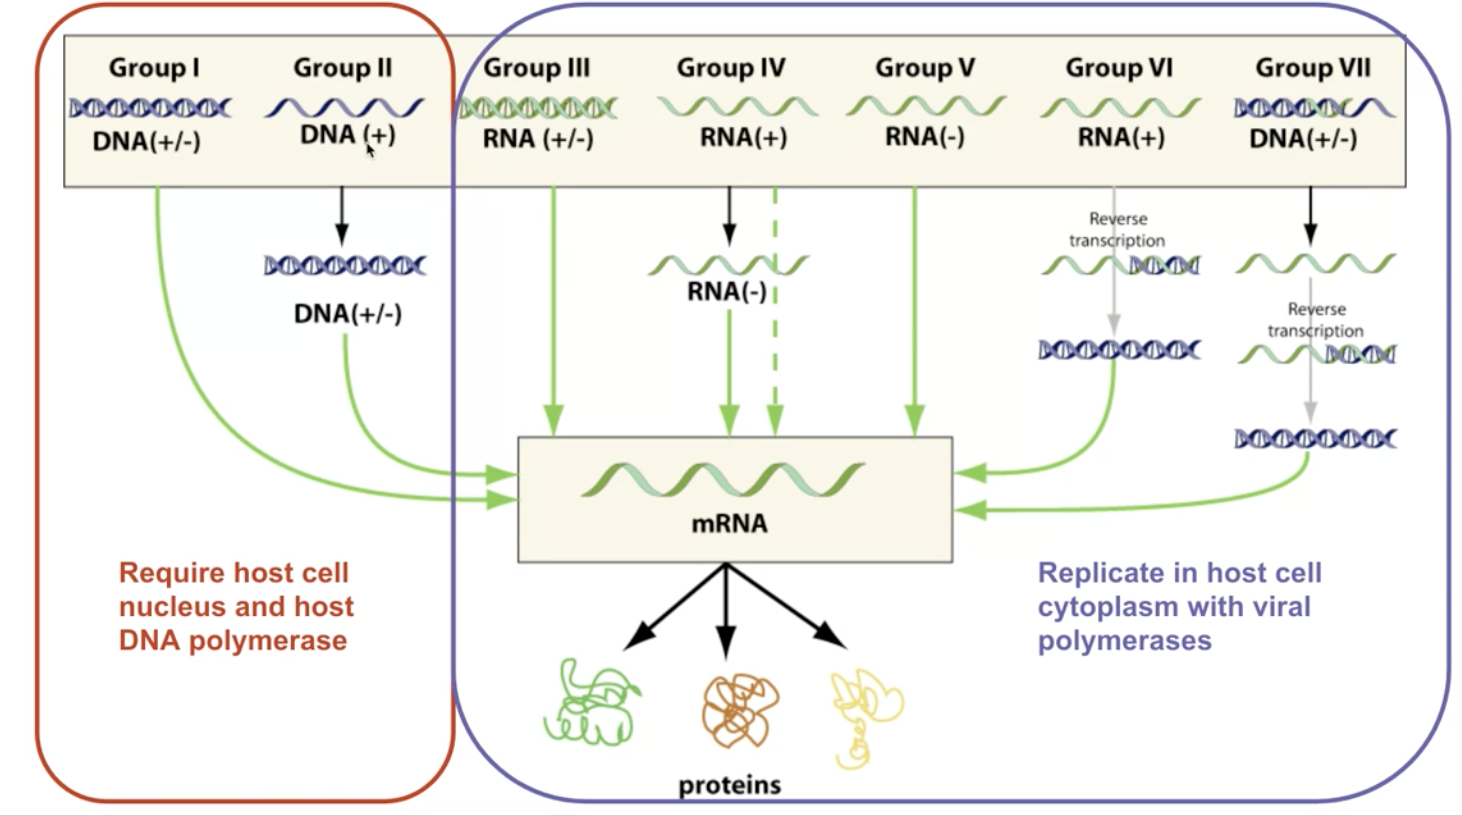
\includegraphics[width=.9\linewidth]{Screen Shot 2020-10-12 at 11.04.53 PM.png}
\caption{Screen Shot 2020-10-12 at 11.04.53 PM.png}
\end{figure}

\textbf{DNA Viruses}

\emph{How are viral mRNAs produced from the viral genome?}

\begin{itemize}
\item Viral DNA enters, through RNA polymerase II in the host cell, mRNA is
produced
\item mRNAs then read by ribosomes, and there we go
\end{itemize}

\emph{What serves as the templates for viral genome replication?}

\begin{itemize}
\item Viral DNA serves as template for host cell DNA polymerase
\item Viral genome copied repeatedly
\item Virus, then, \textbf{will be replicated within the nucleus} due to it needing
the polymerase to copy DNA
\end{itemize}

Except! Poxvirade carry their own polymerase, so they replicate in the
cytoplasm.

\begin{figure}[htbp]
\centering
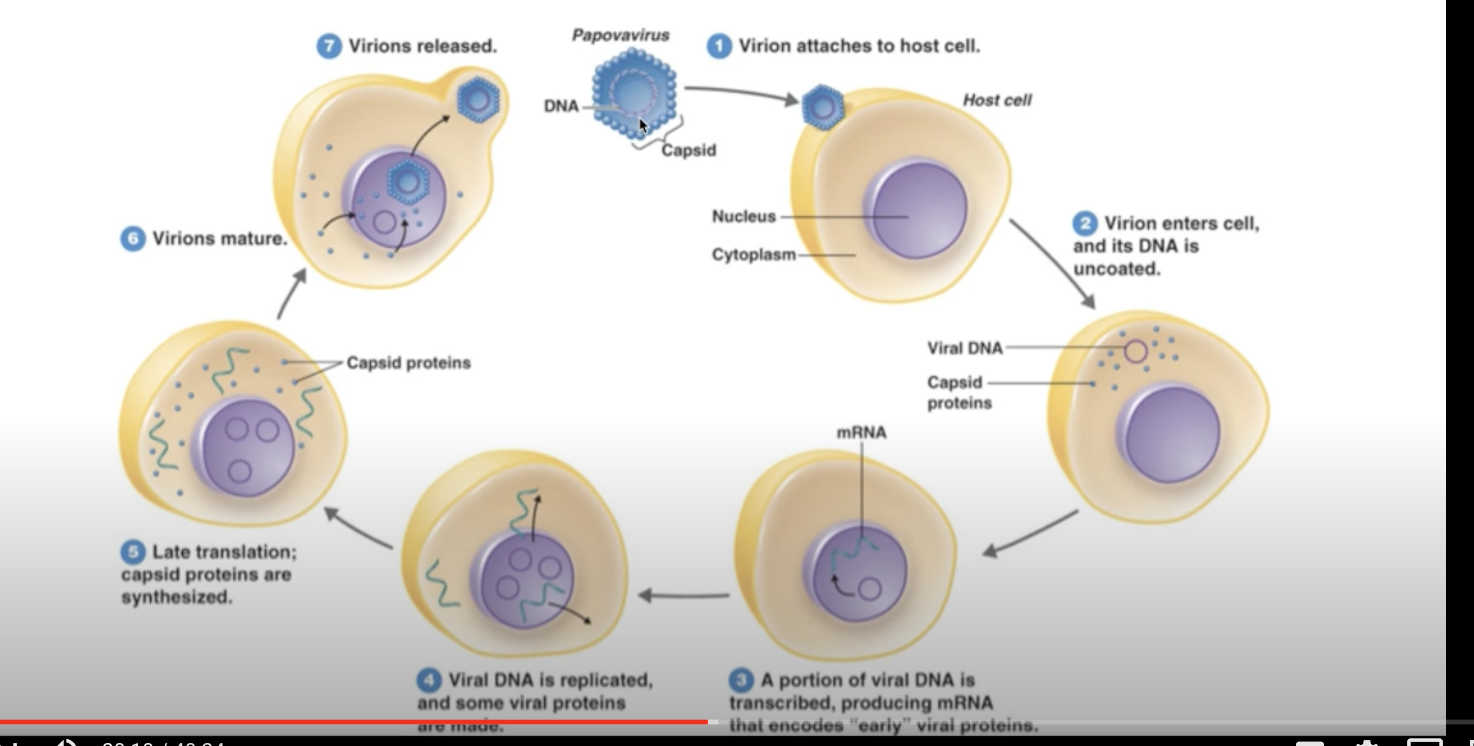
\includegraphics[width=.9\linewidth]{Screen Shot 2020-10-12 at 11.09.46 PM.png}
\caption{Screen Shot 2020-10-12 at 11.09.46 PM.png}
\end{figure}

\textbf{RNA Viruses}

\emph{How are viral mRNAs produced from the viral genome?}

\begin{itemize}
\item +Strand: reproducable RNA => could be directly translated by the
ribosomes
\item -Strand RNA: useless template RNA (less easy to be detected)

\begin{itemize}
\item Need to be processed by RDRP (RNA-dependent RNA Polymerease)
\item Once entered the cell, RDRP goes to work copying -Strand RNA to
+Strang RNA
\end{itemize}

\item double-stranded RNA viron => (+, a.k.a. sense)

\begin{itemize}
\item +-stranded RNA => same idea as above

\item \begin{itemize}
\item strand RNA => virus comes with RDRP that convert -ssRNA to +ssRNA.
Then, same idea as above.
\end{itemize}
\end{itemize}
\end{itemize}

\emph{What serves as the templates for viral genome replication?}

\begin{itemize}
\item RNA viruses does not need host-cell polymeraese to copy RNA
\item They come with polymerase that\ldots{}

\begin{itemize}
\item with dsRNA; takes +ssRNA and makes -ssRMA; combining the two to
produce dsRNA
\item with +ssRNA, takes +ssRNA and makes temporary -ssRNA which makes
more +ssRNA
\item with -ssRNA, takes -ssRNA, and makes temporary +ssRNA, which makes
-ssRNA
\end{itemize}
\end{itemize}

\begin{figure}[htbp]
\centering
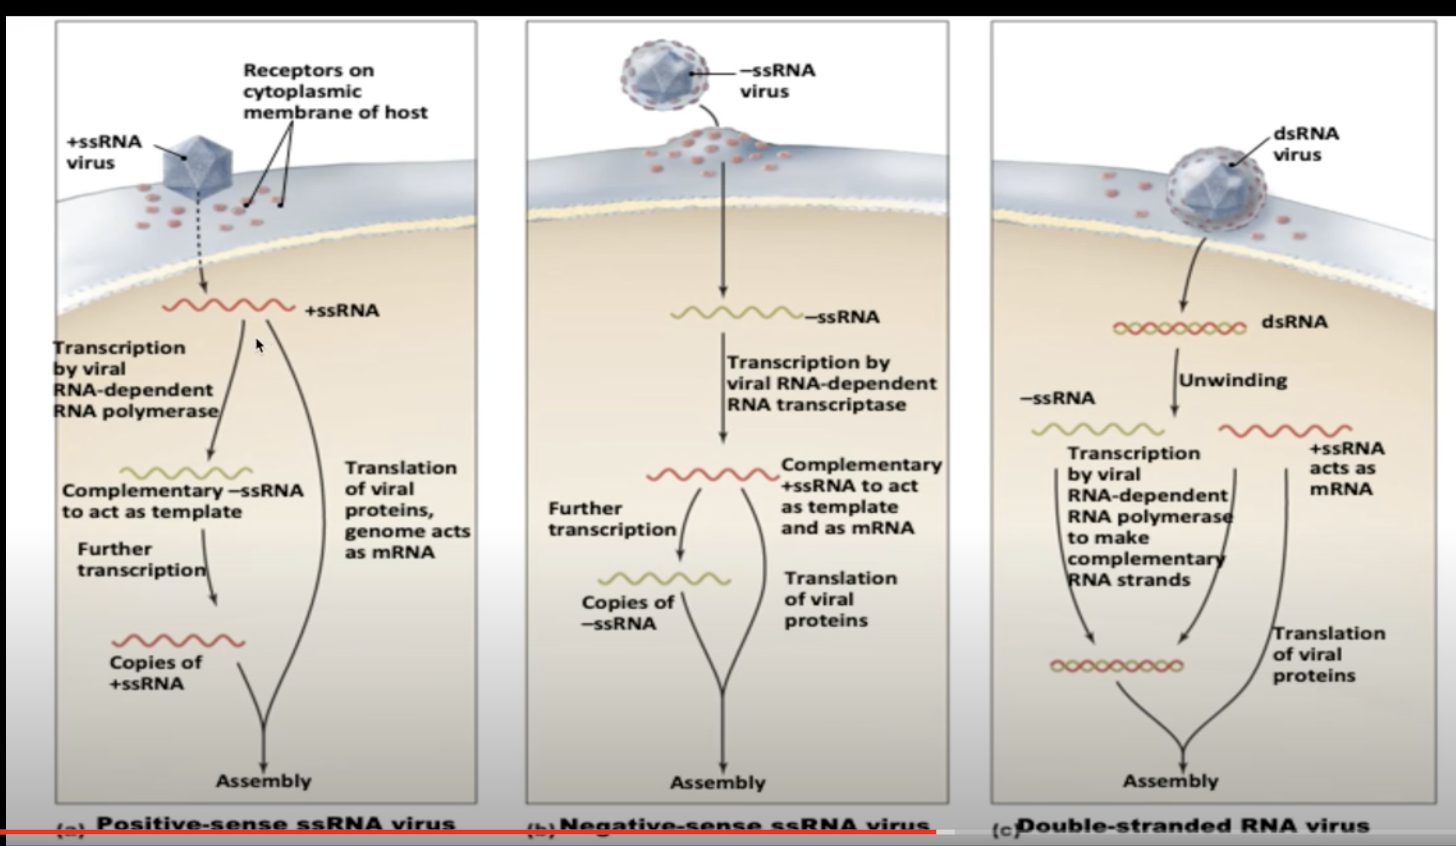
\includegraphics[width=.9\linewidth]{Screen Shot 2020-10-12 at 11.14.30 PM.png}
\caption{Screen Shot 2020-10-12 at 11.14.30 PM.png}
\end{figure}

\item Packaging
\label{sec:org31cd6c3}
Does not require ATP. Just sealed in.

\item Viral Exis
\label{sec:orgce9fd5d}
\textbf{Lysis}

Replicate so much that the membrane burst.

\textbf{Budding}

Trigger\ldots{}

\begin{itemize}
\item Trigger extocytosis
\item Meanwhile, send virus's own spikes to the membrane
\item On exit by extocytosis, steal a part of the newly-spikey membrane with
it to serve as new casing
\end{itemize}
\end{enumerate}

\subsubsection{Viral Genetic Shift + Viral Genetic Drift}
\label{sec:org855c860}
\textbf{Shift} => whole segments of genome exchange abruptly as two flu viruses
infect the same cell to create a new strand.

\textbf{Drift} => single/groups of nucleotides flip slowly over time.

The former is an environment-dependent process, where the latter is able
to be modeled as it is due to transcription mistake.

\subsubsection{Retroviruses + How to Stop Them}
\label{sec:org83b3253}
\textbf{Viruses that have the ability to intergrate into the chromosomes of the
host cell}

\begin{enumerate}
\item Early Events
\label{sec:orgaae2435}
\begin{itemize}
\item Viruses is uncoated, and uses an enzyme called reverse transcriptase
to turn ssRNA to cDNA, and finally into dsDNA
\item Then, the enzyme integrase threads the viral dsDNA into the cell's
nucleaus
\item HIV protease cuts HIV polyproteins into individual parts ready for
budding
\end{itemize}

\item Late Events
\label{sec:org7c90343}
\begin{itemize}
\item Proviral region is transcribed slowly whenever ribosome comes across
it by the host DNA polymerase II to make viral proteins + replicate
the viral genome
\item Components are later exported, assembled, and slowly released through
budding
\end{itemize}

To make this happen, the virus needs\ldots{}

\begin{itemize}
\item \textbf{Reverse Transcriptase}

\begin{itemize}
\item Transcript RNA to double-stranded RNA
\item Take double-stranded RNA to turn into DNA
\end{itemize}

\item \textbf{Integrase}

\begin{itemize}
\item Force insert the DNA into the genome of the host cell
\end{itemize}
\end{itemize}

And because of the fact that viral DNA is now in cellular DNA, these
viruses' DNAs are hard to get rid of.

And this is why we can't cure HIV.

Virus, in this case, spread through cell duplication

\begin{itemize}
\item Proviral region on the DNA, every time the ribosome comes across it,
makes a new viron
\item These components are then assembled, sent, etc. as usual
\item Because of the fact that the ribosome needs to, well, come across the
bit of DNA for this to work, the virons are made slowly by “trickling
out.
\end{itemize}

\begin{figure}[htbp]
\centering
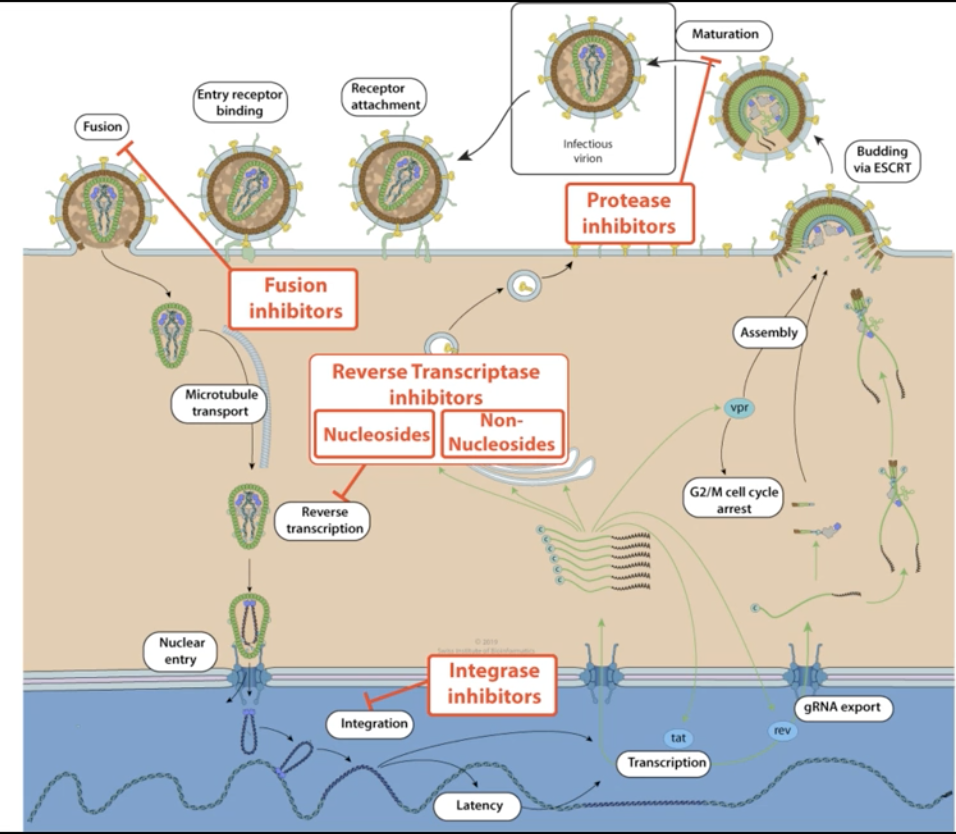
\includegraphics[width=.9\linewidth]{Screen Shot 2020-10-12 at 11.22.35 PM.png}
\caption{Screen Shot 2020-10-12 at 11.22.35 PM.png}
\end{figure}

\textbf{Preventing Retroviruses}

\begin{itemize}
\item Prevent Fusion \texttt{gp120}, \texttt{gp41}, \texttt{CCR5}
\item Prevent reverse transcription \texttt{RT}
\item Prevent intergration via intergrease \texttt{IN}
\item Prevent viron maturation \texttt{PR}
\end{itemize}

\begin{figure}[htbp]
\centering
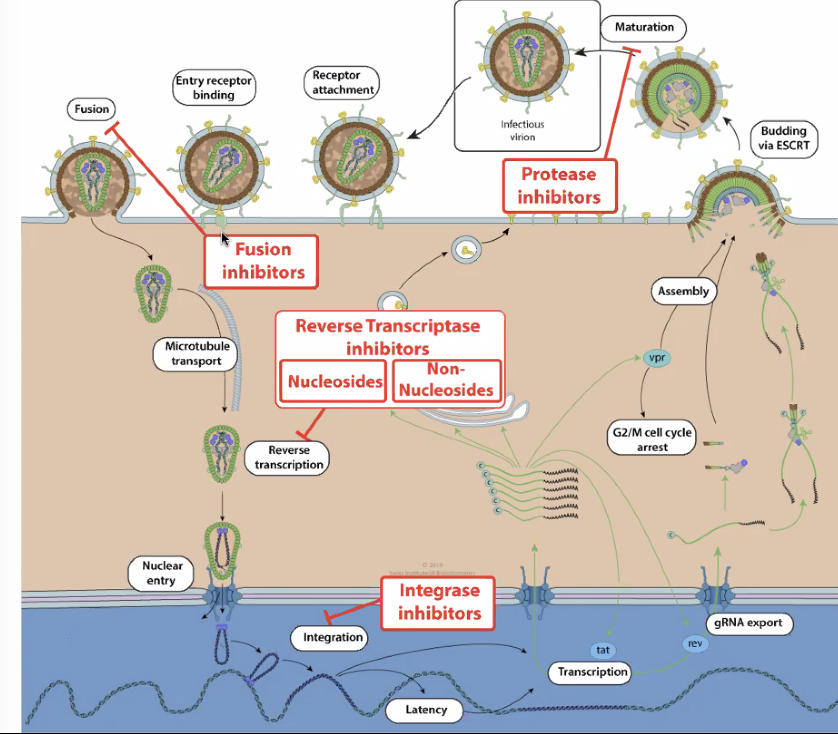
\includegraphics[width=.9\linewidth]{stophiv.png}
\caption{stophiv.png}
\end{figure}

\begin{itemize}
\item Most advanced: HAART (Highly-Active Anti-Retroviral Therapy)

\begin{itemize}
\item Cocktail drug works together for inhibition
\item Two drugs to stop intergration, one to stop protease (viron
maturation)
\item Could develop resistance
\end{itemize}
\end{itemize}
\end{enumerate}

\subsubsection{Viral Genome vs Mutation Rate}
\label{sec:orgdcba344}
\begin{figure}[htbp]
\centering
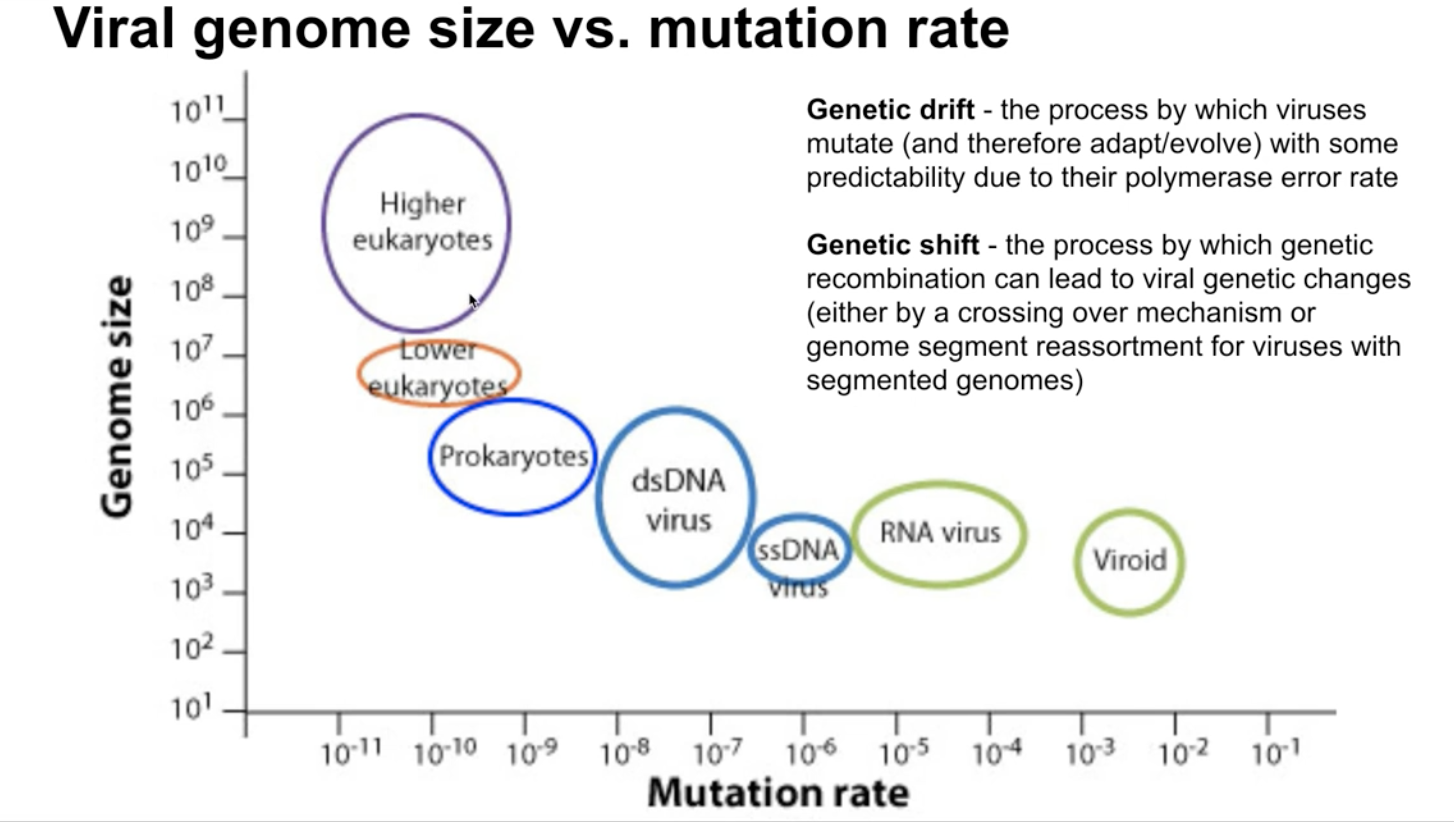
\includegraphics[width=.9\linewidth]{Screen Shot 2020-10-12 at 11.24.39 PM.png}
\caption{Screen Shot 2020-10-12 at 11.24.39 PM.png}
\end{figure}

\begin{itemize}
\item RNA viruses could mutate more because it does not have checks
\item More complex+largest viruses harder to mutate
\end{itemize}

\textbf{Genetic drift} --- viruses mutate due to polymerase error

\textbf{Genetic shift} --- viruses recombinate without mutating by
crossing-over mechanism or genome segment reassortment. Think! the flu

\subsection{Why are viruses bad}
\label{sec:orgc3e939b}
Damage host cells/tissues by\ldots{}

\begin{itemize}
\item Reducing gene expression capacity
\item Depleting cellular resources
\item Causing cell lysis (to explode)
\item Promoting tumorigenisis --- cancer
\item Creating damaging immunological response
\end{itemize}

\subsection{Preventing Viruses}
\label{sec:org1300a08}
Let's talk about \textbf{Remdesivir}! A drug developed by Pfizer that's used to
combat Ebola + influenza viral replication.

Modified nucleotide triphosphate which adds onto the RNA strand copied
by the RNA-Dependent RNA Polymerase carried by viruses

\begin{itemize}
\item Pretends + gets inserted as a nucleotide
\item Once added onto the RNA chain, jams further actual nucleotides from
being inserted
\end{itemize}

\emph{Could} but usually does not jam up normal RNA polymerase which does
normal transcription

\begin{itemize}
\item Inhibiting transcription in the short term won't kill you immediately
\item So, we hurt normal cell transcription a little in order to rid of the
virus
\item Need hospital treatment for regular and safe dosing for this exact
reason
\end{itemize}

\section{CN10212020}
\label{sec:org130d250}
\subsection{Making Proteins, a guide}
\label{sec:org0872433}
\textbf{Genetic Code} => "nucleotide code" found in the DNA that helps make
protein. There are two parts of this: translation and transcription.

\begin{itemize}
\item The process of \textbf{Transcription} involves taking the DNA, separating it,
and copying its corresponding pairs to RNA
\item The process of \textbf{Translation} involves taking the RNA and making
proteins.
\end{itemize}

Occasionally, the RNA is what we want to end up with, so then obviously
we no longer need the process of Translation.

\subsubsection{Transcription => converting DNA to mRNA}
\label{sec:orgb964f0a}
\begin{itemize}
\item Done by RNA Polymerase Enzyme
\item Rip apart hydrogen bonds using DNAse enzyme
\item Read one side ("template strand", a.k.a. noncoding strand) of the
double helix, recognizing each nucleotide
\item Pluck the correct corresponding nucleotide out of the nucleus

\begin{itemize}
\item G->C
\item C->G
\item A->*U*
\item T->A
\end{itemize}

\item Prokaryotes lack membrane-bound nucleus (or any organelle)
\end{itemize}

\definition{Gene}{information that successfully encodes a functional protein or a functional catalytic RNA}
RNAs could also be catalysts!

\begin{itemize}
\item "Promoter"s denotes beginning of a gene. "Terminator"s denotes the end
of gene.
\end{itemize}

\textbf{Starting Transcription} * Series of utility "factors" proetins begin to
assemble to call the attention of RNA polymerase. (\#how + \#when does
this happen? \#ASK) * RNA polyamerase binds to the Sigma Subunit => form
a holoenzyme to unwind DNA * Sigma subunit informs the enzyme where to
find a promoter (beginning of binding) * "Enhancer" gene sequences help
bind with activator proteins to help attract RNA polymerase II

\textbf{Promoters}

\begin{itemize}
\item Polymerase Enzyme starts at a promoter (typically found upstream of
the 5' start site) and ends at a terminator

\begin{itemize}
\item Box of TATTAA highlights transcription rate and the start site
\item TFIIA cofactor in RNA recognizes TATTAA box, TFIIB recognizes
C/CG/CG/CGCCC upstream
\end{itemize}

\item Stronger promoters/enhancers => "enhance" "more." i.e. tumor viruses
strengthen promoters for cell growth
\end{itemize}

\textbf{Terminators}

\begin{itemize}
\item Found in the end of the template sequence
\item Two types in prokaryotes

\begin{itemize}
\item Rho-independent terminators --- roll back onto itself, causing the
RNA to terminate and mRNA to be release
\item Rho-dependent terminators --- activate cofactor named rho + unwind
the transcribed RNA-DNA hybrid
\end{itemize}

\item In Eukarotes

\begin{itemize}
\item Pol I genes --- transcription stopped through termination factor by
unwindng the transcribed RNA-DNA hybrid
\item Pol II genes --- don't stop until the end, but a polymerase has a
"cleavage" mechanism that clips the end out using a poly(A) tail
consensus sequence
\end{itemize}
\end{itemize}

\subsubsection{Before we continue, two words}
\label{sec:org5e3d75f}
\begin{itemize}
\item \emph{Non-coding sequence}: metadata for DNA for the processors
\item \emph{Coding sequence}: DNA content for amino-acid production
\end{itemize}

\subsubsection{mRNA processing => splicing mRNA}
\label{sec:org8daabcb}
Pre-process the mRNA.

\textbf{Prokaryotes does not do this!} Prokarotes' coding sequence always makes
a full protein, so we just start at promoter and end at terminator and
make a protein!

In Eukaryotic DNA\ldots{}

Between Promoter and Terminator, \textbf{Exon} and \textbf{Intron} alternate. Exon is
coding, whereas Intron is non-coding and works as metadata.

After reading the intron, they are spliced out during mRNA processing =>
done by the "splicesome". The mRNA, after splicing, is "capped and
tailed" to mark pre-processing completion, at which point they leave the
nucleus + go to the ribosome.

\begin{itemize}
\item Begin by assembling helper proteins at intron-exon borders => "slicing
factors"
\item Other helping factor proteins come together and form the "splicesome"
to do the splicing
\item Splicesome splices by bringing exon ends together
\item After it's done, the splicesome disintergrates
\end{itemize}

\subsubsection{Translation => RNA-directed polypeptide synthesis}
\label{sec:org960d367}
Mature mRNA sent to ribosome. mRNA must travel to the cytoplasm in the
Eukarotes to catch the RNA, whereas in prokarotes they don't have to go
anywhere.

Ribosomes has two units: 50S unit + 30S unit => they come together
whenever a mRNA needs it. Each contained specialized rRNA + tTRNA to
catalyze attachment of and carry amino acids + adapt the incoming mRNA
respectively.

\textbf{Note! The beginning of mRNA is not translated.} There a portion on the
5' end of the mRNA (starts with AGGAGG) --- about 170 nuclotides in
humans, and shorter in bacteria --- that's called UTR (untranslated
region.) This region helps ribosomes bind to it + stablize the binds.

\begin{itemize}
\item 3 protein factors IF1, IF2, IF3 forms a complex for transcription by
binding to a subunit on the ribosome
\item Methionine-carrying tRNA binds to the start of the mRNA, which forms
the initiation complex. This is typically removed after translation if
not coded for (f M-A amino acid pair coded for, methonine removed; but
if M-L pairs coded for, methonine not removed.)
\item A-site: translates mRNA to tRNA --- anti-codon pairs
\item P-site: amino acid dumped from tRNA to the actual chain being built
\item Spent tRNA ejected to the E-site, which is then recycled
\item Catalyst tRNA combines with rRNA to catalyze amino acid peptide bond
\item Each codon (group of 3 units in tRNA), matches a specific
\href{KBhBIO101AminoAcids.org}{KBhBIO101AminoAcids}
\end{itemize}

Smaller ribosome unit grabs, larger attaches + forms amino acid

After the amino acids are assembled, it's time for
\href{KBe2020bio101refProteinFolding.org}{KBe2020bio101refProteinFolding}.
See also \href{KBhBIO101Proteins.org}{KBhBIO101Proteins}.

=> Shaperones fold proteins, and if its finds proteins impossible to
fold, it flags it using ubiquitin to send to the garbage

\noindent\rule{\textwidth}{0.5pt}

Eukarotic gene expression is regulated at many stages --- prevents error

\begin{figure}[htbp]
\centering
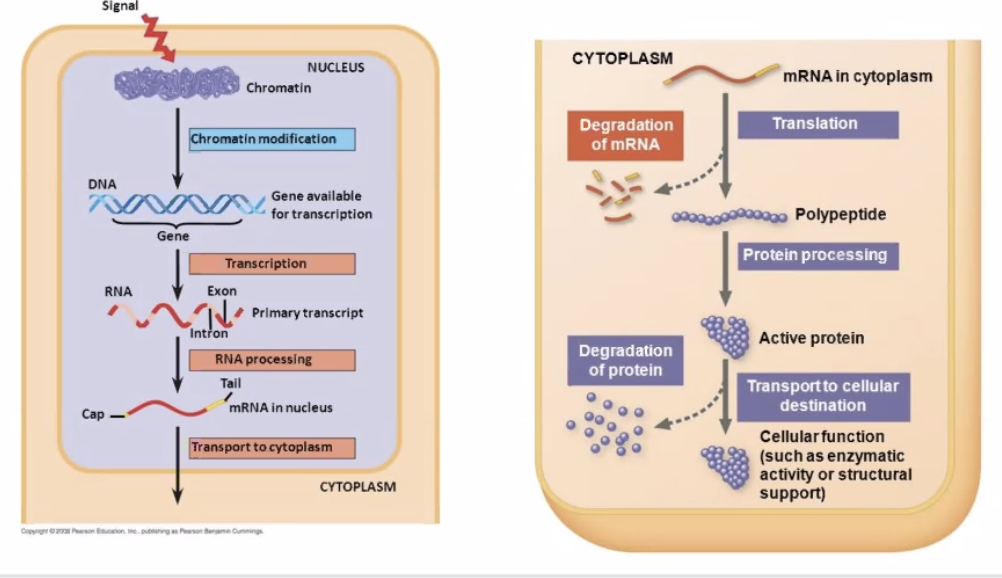
\includegraphics[width=.9\linewidth]{preprocessing.png}
\caption{preprocessing.png}
\end{figure}

\begin{itemize}
\item Viral proteins are usually easy to assemble
\end{itemize}

\begin{figure}[htbp]
\centering
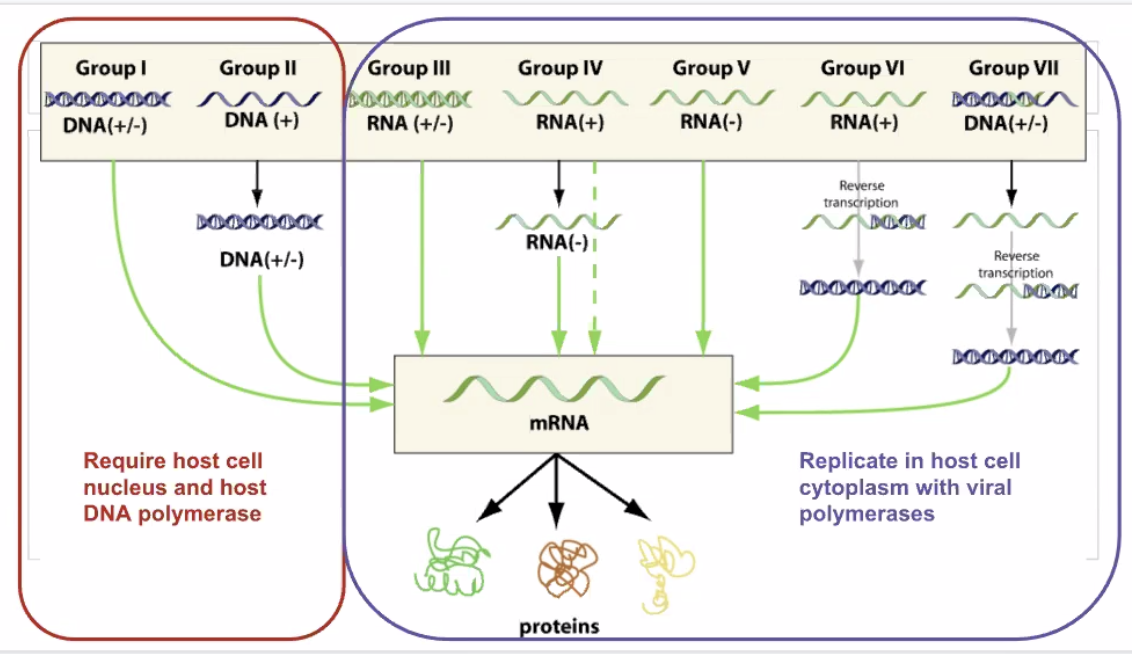
\includegraphics[width=.9\linewidth]{Screen Shot 2020-11-02 at 2.48.22 PM.png}
\caption{Screen Shot 2020-11-02 at 2.48.22 PM.png}
\end{figure}

In Prokarotes, there are less steps.

Between the promoter and the actual coding DNA, there is a region named
\emph{operator} that allows three types of regulatory molecules to bind to it
to alter how the gene is transcribed, namely:

\begin{itemize}
\item \textbf{Repressors}: proteins that suppress transcription
\item \textbf{Activators} are proteins that increase the transcription
\item \textbf{Inducers} catalyses repressors or activators --- making either a
strenthened activation or repression acting in conjunction with the
other regulator
\end{itemize}

\textbf{Question: how are proteins made in the viral genome}

\begin{itemize}
\item No viruses produce ribosomes
\item Ribosomes become centrally important for the virus
\item What serves as the template to make new virus copies
\end{itemize}

Viruses attempt to overwhelm the enzyme to entry.

\begin{itemize}
\item \textbf{DNA Polymerase} takes DNA and makes more DNA

\begin{itemize}
\item Duplicates cell DNA
\item Could be hijacked during cell cycle to duplicate DNA viruses
\item DNA viruses may also carry their DNA Polymerease to not wait for the
cell cycle
\end{itemize}

\item \textbf{RNA Polymerease} takes DNA and makes mRNA

\begin{itemize}
\item Have lower fidelity with an error about 1/100,000
\item Hence why safety mechanism needed
\end{itemize}
\end{itemize}

\textbf{Capping and Tailing} * 3' end => AAAAAA tail (using poly-adenine
tailing enzyme) * 5' end => GGGGGG cap (using guanine-capping enzyme)

\textbf{DNA} viruses are "less complex", in that as long as they are able to
get into the nucleaus, the rest would just be the body's work
automatically.

\subsubsection{List of Kool Proteins}
\label{sec:org0978fac}
\begin{center}
\begin{tabular}{ll}
Name & Function\\
\hline
RNA Polymerase & \emph{transcripts}: takes DNA and turns into mRNA\\
DNA Polymerase & \emph{replicates}: takes DNA and makes more copy of it\\
RNA-Dependent RNA Polymerase & \emph{replicates}: takes RNA and makes more copy of it. Basically only viruses use it.\\
Promoter & \emph{signals}: DNA signal of the start of the DNA.\\
Terminator & \emph{signals}: DNA signal of the end of the DNA.\\
\end{tabular}
\end{center}

\noindent\rule{\textwidth}{0.5pt}

\subsection{DNA Replication and the Cell Cycle}
\label{sec:org312eead}
\subsubsection{So, why do cell divide}
\label{sec:orga441b49}
\begin{quote}
The ability to produce organisms more of their kind is one
characteristic that best distinguishes living things from nonliving
matter
\end{quote}

Viruses + Organelles challenge this definition => they are symbiotic and
cannot reproduce on their own. We tend to think that cells

\begin{itemize}
\item Everyday, 50-70 Billion die => \textbf{programmed cell death}
\item To compensate this, Mitosis (cell division) happen

\begin{itemize}
\item Cell divide in opposite directions
\item Two strands ANTIPARALLEL to each other
\end{itemize}
\end{itemize}

\subsubsection{Levels of DNA structure}
\label{sec:org99ca120}
\begin{itemize}
\item DNA Double Helix => Unwrapped, raw DNA
\item Histones => coiler proteins at which DNA coils around

\begin{itemize}
\item Four histones
\item H3, H4, H2a, H2b wraps, H1 seals the four together
\item Each protein has 1.65 wraps
\end{itemize}

\item Nucleosomes => stack of 2 histone groups to create a spool of 8
histone proteins wrapping DNA
\item Nucleosomes wraps around into a large fiber called "chromatin"
\item A pair of chromatin entangle to form a chromasome
\end{itemize}

\subsubsection{Cell divison process}
\label{sec:orge8fdd17}
\begin{itemize}
\item Chromesomes line up in equator
\item Each chromesome has two chromatid exactly the same
\item Microtubials to pull chromesomes appart connected to kinecore, a joint
in the chromatid
\item Kinetore senses tension, and when it is correct, molecules are sent
down the microtubials to send a split signal
\end{itemize}

\begin{figure}[htbp]
\centering
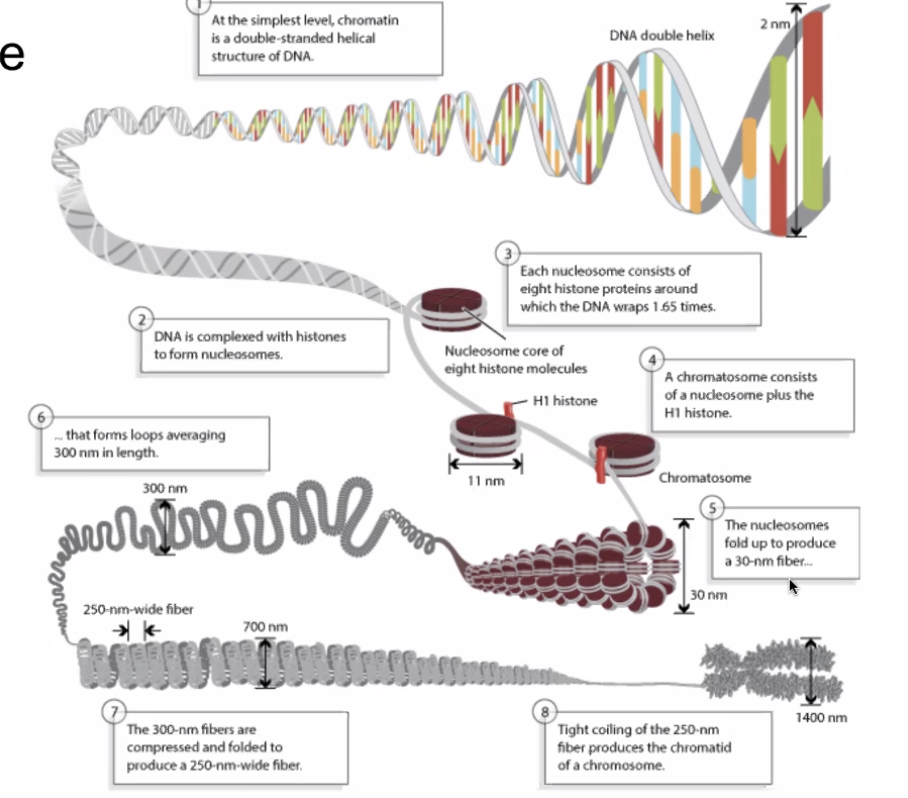
\includegraphics[width=.9\linewidth]{levelsofdna.png}
\caption{levelsofdna.png}
\end{figure}

\begin{figure}[htbp]
\centering
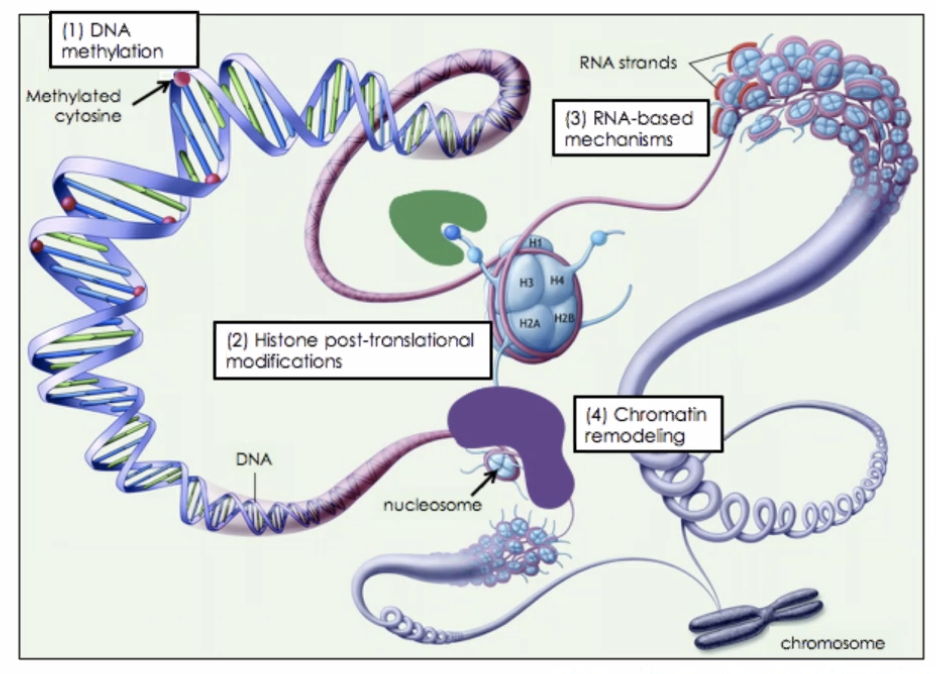
\includegraphics[width=.9\linewidth]{histones.png}
\caption{histones.png}
\end{figure}

\textbf{Most cell division results in genetically identical daughter cell}

Each cell, once specialised, chooses what parts of their chromasome to
unwrap + permanently wrap.

Difference in transcription results in different phenotypes.

Sperm + Egg (imcomplete cells) combine together to form a "zygote" => a
single cell. Each person is from a zygote.

For Eukarotes, cells divide using Mytosis.

\href{https://docs.google.com/document/d/1TIrgR9VSV3attTK\_QP-AOCs33mMoBP0Cz7DQXysKoD0/edit}{Paul's
Cell Cycle Primer}

\begin{figure}[htbp]
\centering
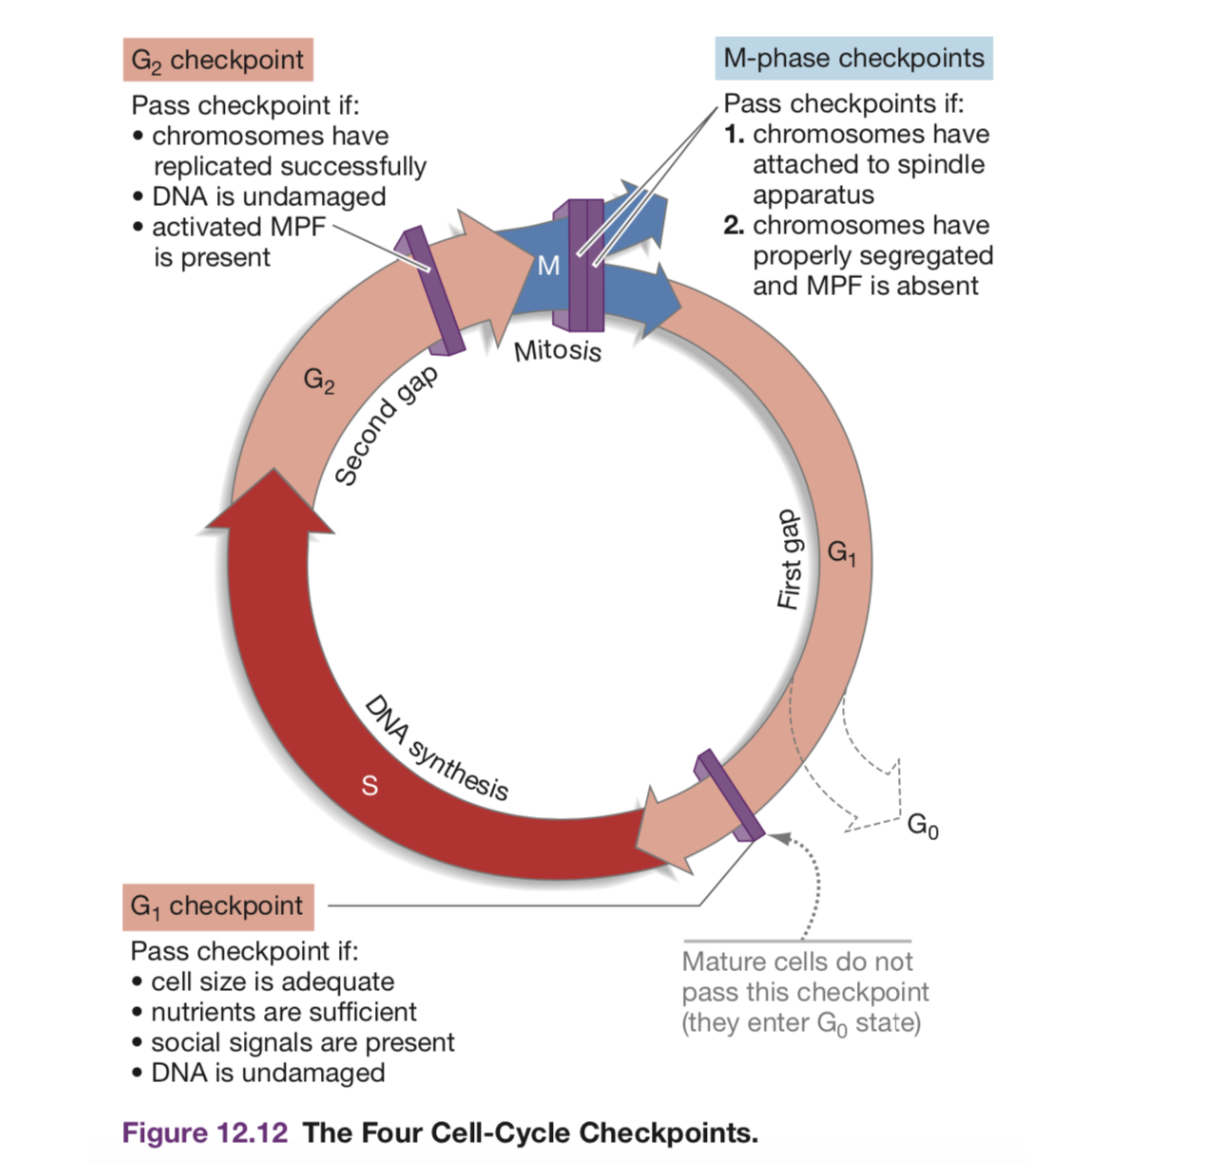
\includegraphics[width=.9\linewidth]{Screen Shot 2020-11-09 at 3.16.12 PM.png}
\caption{Screen Shot 2020-11-09 at 3.16.12 PM.png}
\end{figure}

\subsubsection{Major Cell Cycle Parts}
\label{sec:orgf773318}
\begin{itemize}
\item G1 => Rest Phase, Gap 1

\begin{itemize}
\item May hit s.a. to volume checkpoint => if ratio too big, the cell is
too big
\item May hit diffusion checkpoint => larger cells would need to work
harder to transport things to the centre
\end{itemize}

\item S => S Phase, duplicate DNA. 150 mins
\item G2 => Rest Phrase, Gap 2. The pairs of DNA begins bundling and
condensing; the DNA is also checked upon and verified for consistency
\item M => Mitosis!

\begin{itemize}
\item Prophase: condensation of chromasome
\item Chromatin aligns in the center => (metaphase)
\item A divit (DEFINITION?) forms
\item Two chromatin becomes pulled apart => forming two cells via
cytokenisis (anephase)
\end{itemize}
\end{itemize}

Cell regulators are proteins that manage and sheperard the process of
cell division. They respond to molecular signals throughout the cell and
check for internal signals like DNA damage to control the rate and
progress of cell division.

\begin{figure}[htbp]
\centering
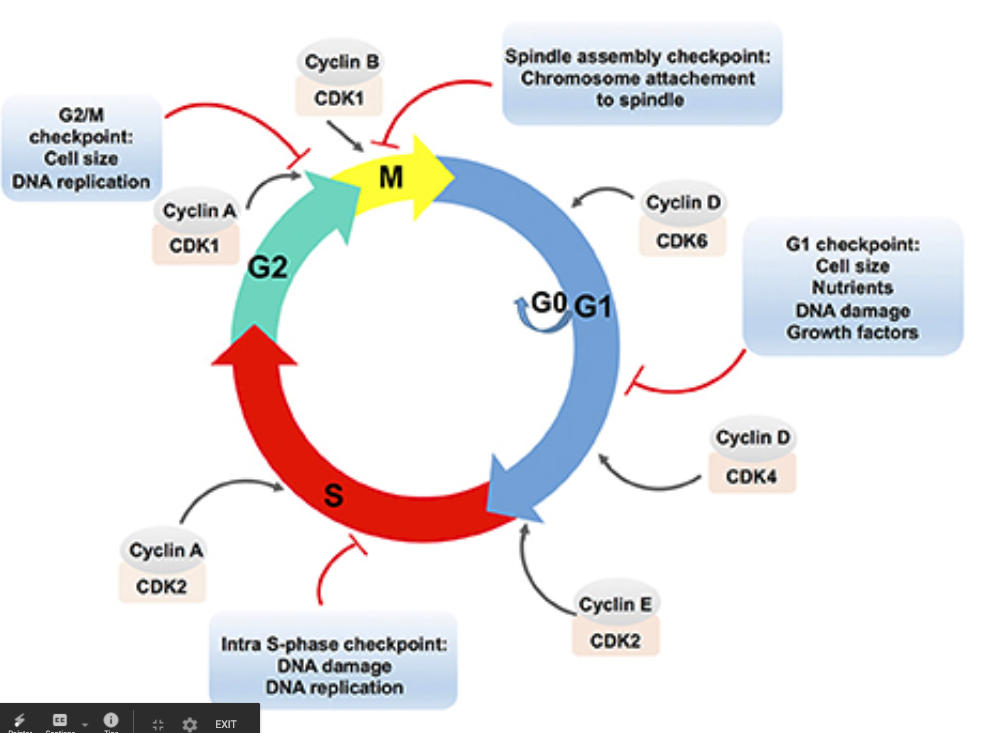
\includegraphics[width=.9\linewidth]{lecellcycle.png}
\caption{lecellcycle.png}
\end{figure}

\subsubsection{DNA Replication Process}
\label{sec:orgc5ad7c3}
DNA replication is known to be "semi-conservative" --- meaning that it
is a process that pairs a synthesized half of the DNA with an original
half of the DNA (i.e. takes the ORIGINAL template strand + makes the NEW
coding strand \& takes the ORIGINAL coding strand + makes the NEW
template strand.)

Because \textbf{polymerases copy uni-directionally} => DNA polyemrease move
along the 3' to 5' DNA to create a copy 5' to 3'. Meaning, the
polymerize is able to add nucleotide onto the 3' end of the DNA.

\begin{itemize}
\item Open the DNA at an arbuiturary point using the Helicase

\begin{itemize}
\item Uses two helicase => one open rightward, and one leftward. The
movement of the helicase opening the DNA is called the "fork
movement"
\item DNA polymerase could only add nucleotides 5' to 3'
\item As helicase open a little bit of the DNA, polymerases rushes to copy
the area that opened

\begin{itemize}
\item In the \textbf{leading} strand (3' to 5'), polymerase will run alongside
the helicase for they are opening and replicating on the same
direction
\item In the \textbf{lagging} strand (5' to 3'), polymerase will wait until the
helicate opens a little segment, and rushes forward and move
backwards

\begin{itemize}
\item NOTE: the lagging strand\ldots{} 1) takes longer to transcribe 2) is
done in small chunks (each "rush forward"). Each chunk is called
an ogazaki fragment
\end{itemize}
\end{itemize}
\end{itemize}
\end{itemize}

\begin{figure}[htbp]
\centering
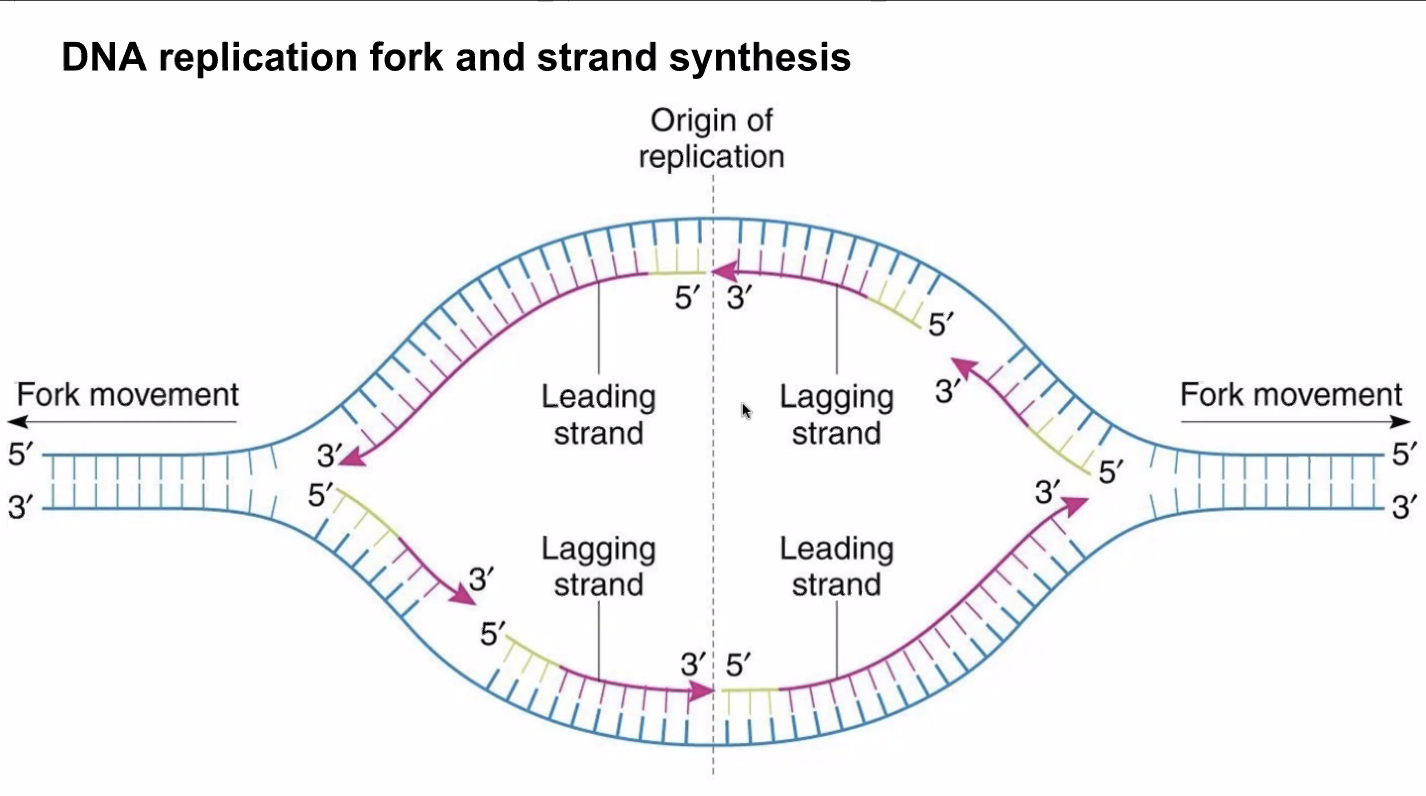
\includegraphics[width=.9\linewidth]{leadinglagging.png}
\caption{leadinglagging.png}
\end{figure}

\begin{itemize}
\item DNA polymersease will REQUIRE a double-stranded area to begin work
from, so Primase synthesize already double-stranded RNA primers that
DNA polymerease could bootstrap to the single-stranded DNA to begin
the replication process (think: create-react-app)

\item DNA polymerse will detect unfitting bonds and remove leftover RNA
primer bootstrap units to repair them in a process called
"proofreading." DNA polimersease is assisted with "glue" ligase to
help the DNA polymerease pick out and replace problematic/unneeded
nucleotides and perhaps their neighbors. This is where the Ogazaki
fragments get joined.
\end{itemize}

Steps of DNA replication, in Paul's words:

\begin{verbatim}
- Many proteins work together in DNA replication and repair. 
The process of DNA replication is semiconservative, such that takes place through complementary base pairing of a template strand of parent DNA. 

- The process of replication begins at the origin of replication, forming a replication fork. The enzyme, helicase, unwinds DNA exposing template strands, primase synthesizes RNA primers to begin the process

- Topoisomerase breaks, swivels, and rejoins the parent DNA to relieve strain caused by unwinding. 

- DNA polymerase is the enzyme that catalyzes the process of complementary base pairing of nucleotides to the template strand. 

- New nucleotide strands always for in the 5’ to 3’ direction, therefore the leading strand forms continuously but the lagging strand is formed in Okazaki fragments (still in the 5’ to 3’ direction) and connected by the enzyme ligase. 

- DNA polymerase is able to proofread pairing, and along with mismatch repair enzymes, DNA is carefully check and repair DNA. 

- The end of a DNA molecule are called telomeres (not in circular genome e.g. bacteria), and shorten during each replication (Hayflick limit). Noncoding, repeating units of nucleotides act as protection from losing essential genetic information by shorting. 
\end{verbatim}
\end{document}
